\chapter{elektrische Komponenten}
\section{der Mikrocontoller}
\subsection*{großer LEGO® Technic Hub:}
Der Hub ist das Steuerungselement des Spike Prime Systems. Er umfasst sechs Ein-/Ausgänge, welche den Anschluss von Peripheriegeräten, wie Sensorik und Aktorik, ermöglicht. Mit einem Micro-USB-Anschluss und Bluetooth wird die Kommunikation mit kompatiblen Endgeräten hergestellt. Der Hub besitzt ein integriertes MicroPython-Betriebssystem mit einem 100-MHz-Prozessor. 
Weitere Ausstattungen sind:
\begin{itemize}
	\item Individuell anpassbaren Lichtmatrix (5x5)
	\item Aufzeigen von wichtigen Informationen und Statusmeldungen
	\item Tasten ermöglichen eine einfache Navigation und Steuerung durch Menüs 
	\item Lautsprecher
	\item 6-achsigen Kreiselsensor
\end{itemize}

\begin{figure}[H]
	\centering
	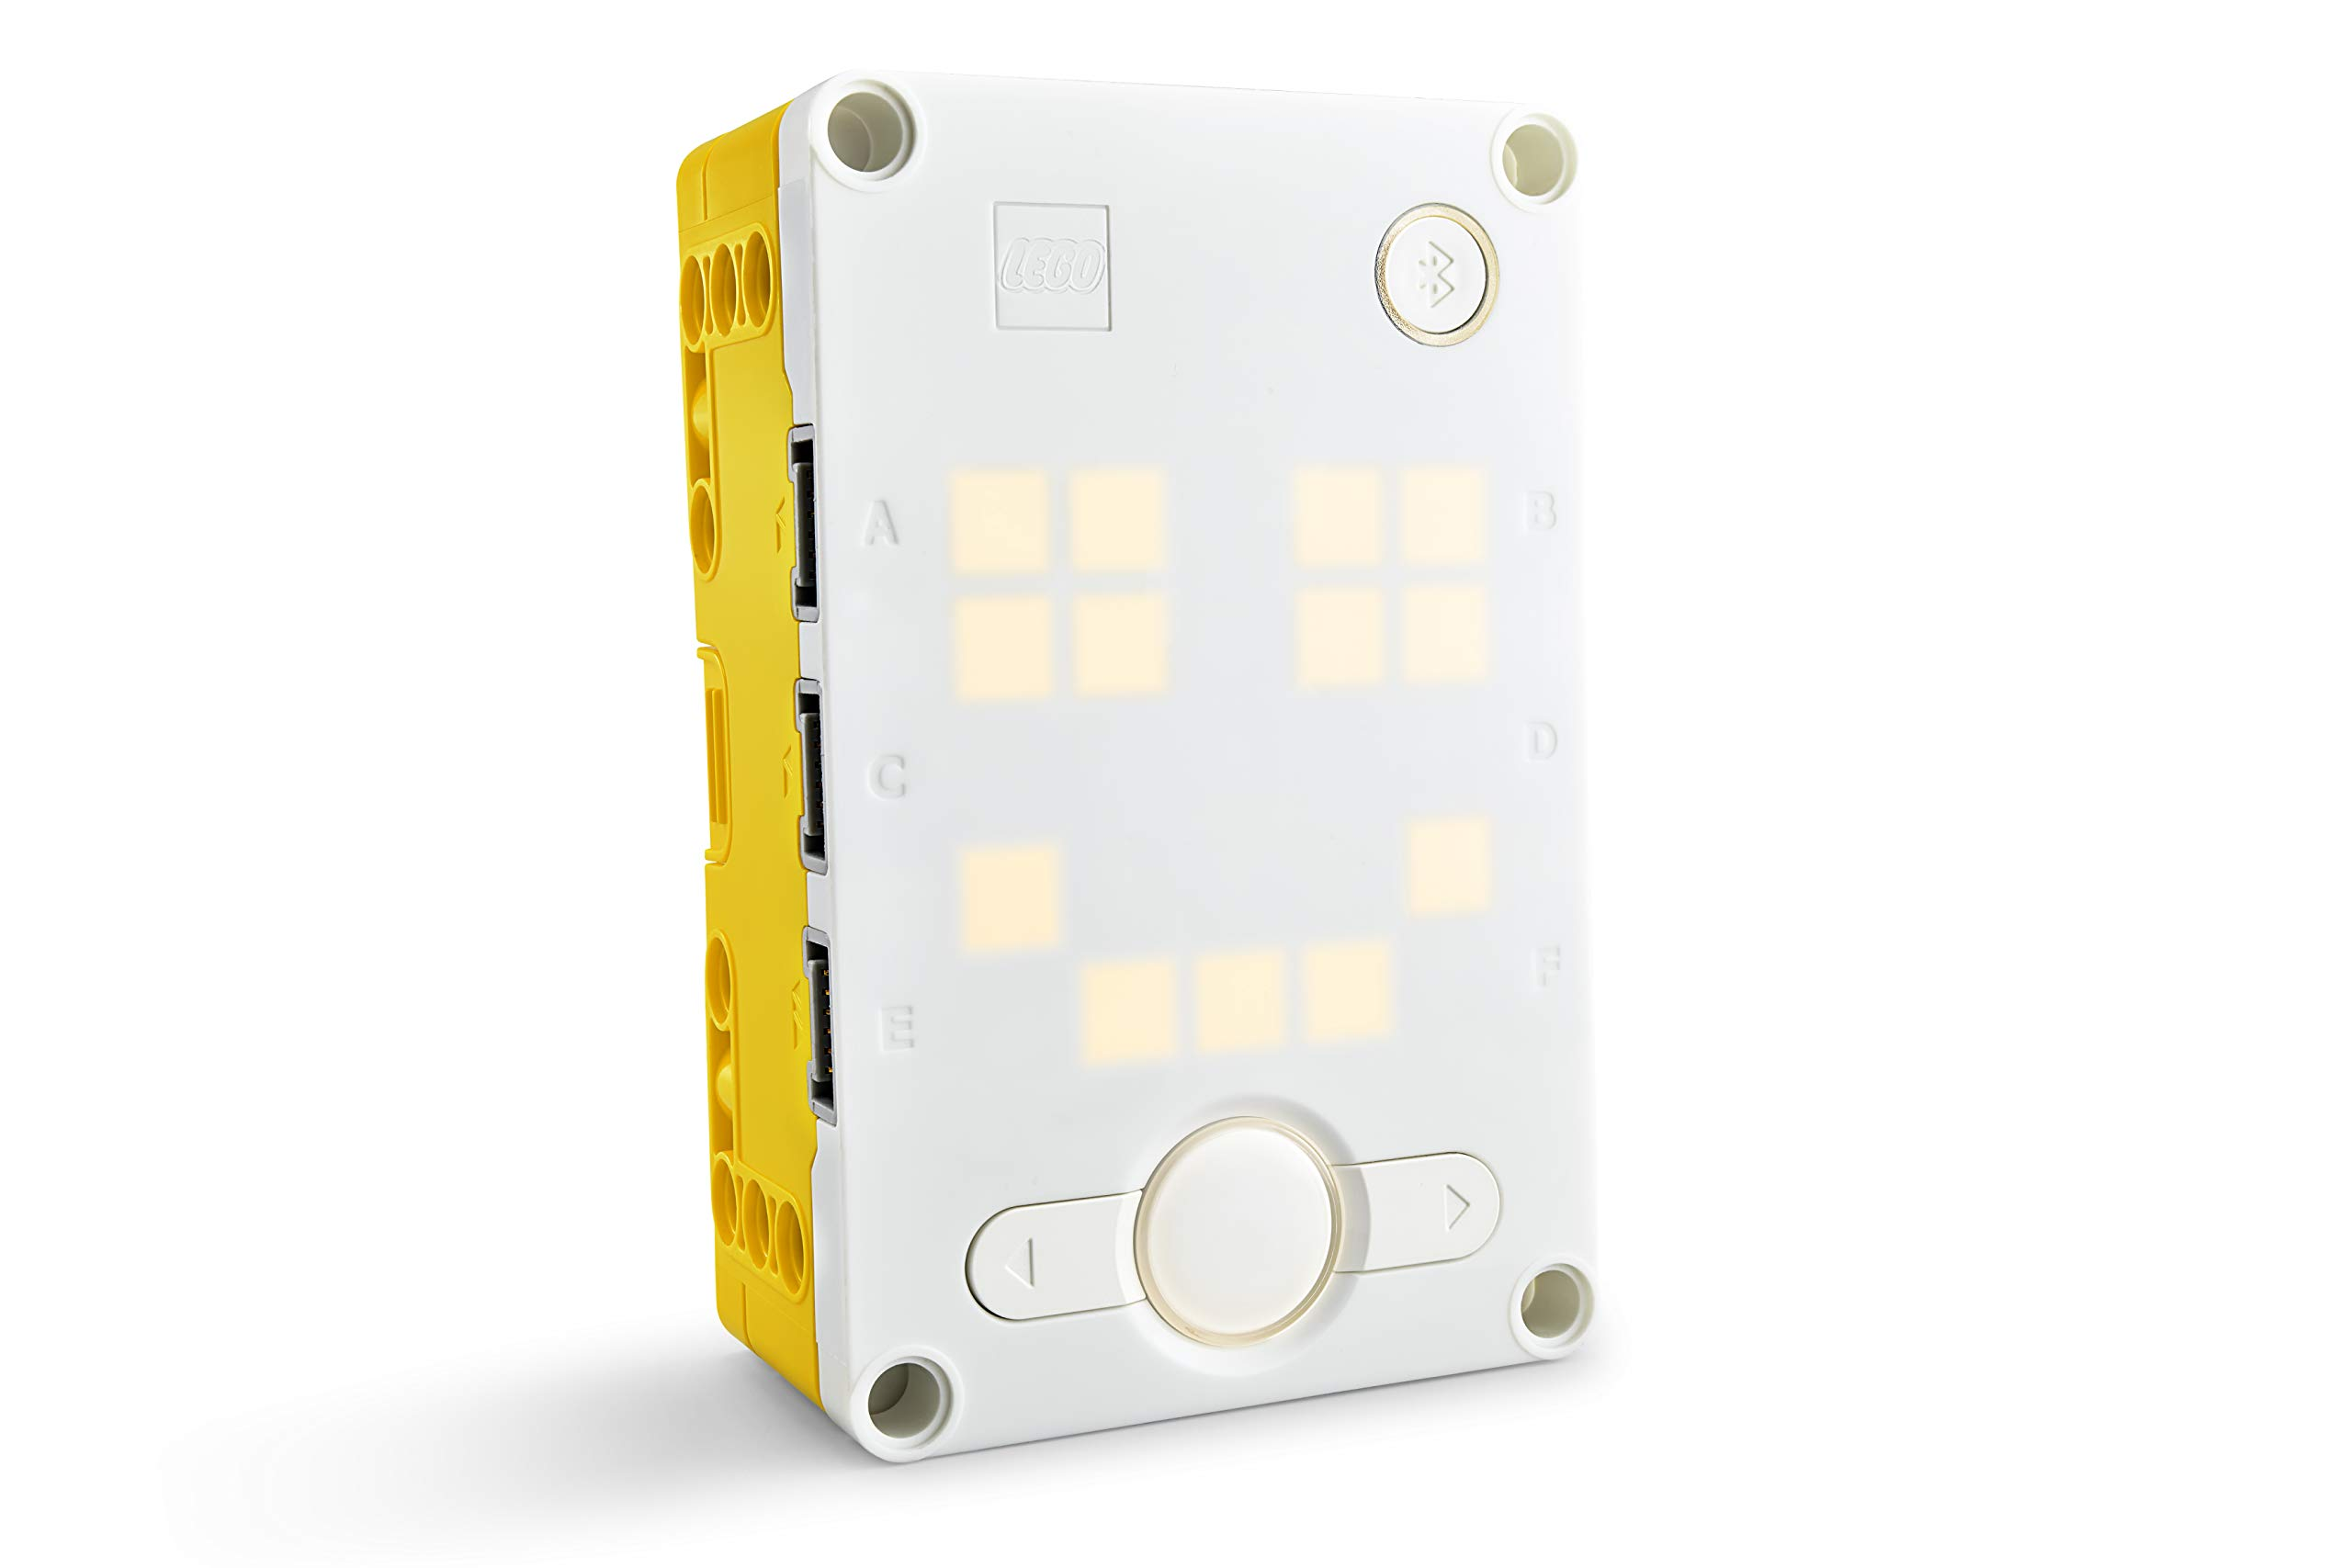
\includegraphics[width=0.4\linewidth]{images/Hub}
	\caption{großer LEGO® Technic Hub}
	\label{fig:hub}
\end{figure}



\section{Sensorik}
\subsection*{LEGO® Technic Farbsensor:}
Dieser Sensor kann durch die Intensität des reflektierten Lichts, welche er durch den eingebauten Lichtring erzeugt, bis zu acht Farben erkennen und unterscheiden (erkennbare Farben: schwarz, blau, rot, weiß, braun, gelb, pink und grün).  Er wird vor allem bei Anwendungen, wie Sortieren nach Farben, Linienverfolgung von farbigen Streifen und zum Ausführen von farbcodierten Befehlen eingesetzt. Um die Farberkennung optimal auf die entsprechende Umgebung anzupassen, wird das Umgebungslicht zuvor ausgewertet.

\begin{figure}[H]
	\centering
	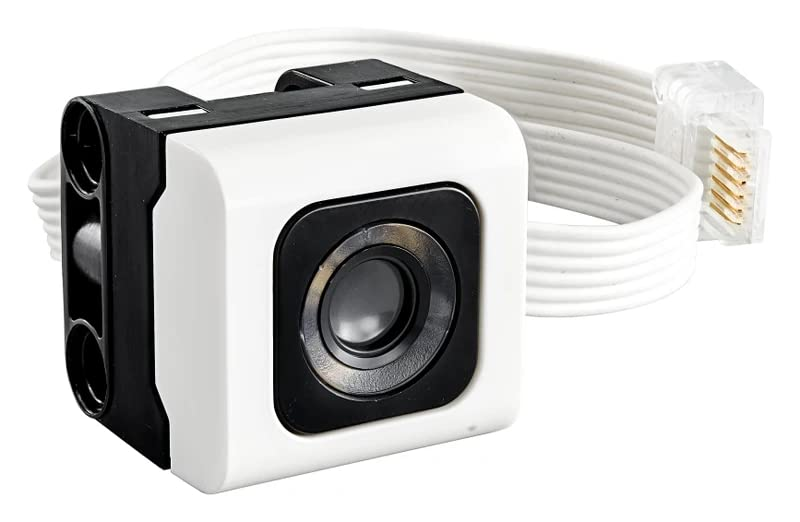
\includegraphics[width=0.4\linewidth]{images/Farbsensor}
	\caption{LEGO® Technic Farbsensor}
	\label{fig:farbsensor}
\end{figure}


\section{Aktorik}
\subsection{LEGO® Technic Großer Winkelmotor}
Für die Bewegungssteuerung wird dieser Winkelmotor mit hoher Drehkraft und präziser Steuerung verwendet. Dieser Motor ist dafür ausgelegt, um schwere und komplexe Konstruktionen exakt in Geschwindigkeit und Position verfahren zu können. Dies wird durch den internen Winkel- und Rotationssensor ermöglicht. Der Anwendungsbereich ist vielseitig, unter anderem wird dies als Antrieb von Rädern, Gelenke, Greifarme, Hebevorrichtungen und Drehscheibe angewandt. Vor allem für Aufgaben, welche eine genau und wiederholbare Aktion ausüben müssen.

\begin{figure}[H]
	\centering
	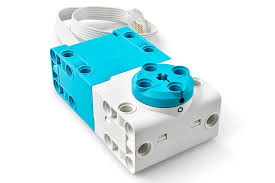
\includegraphics[width=0.4\linewidth]{images/Motor}
	\caption{LEGO® Technic Großer Winkelmotor}
	\label{fig:motor}
\end{figure}
